


%%%%%%%%%%%%%%%%%%%%%%%%%%%%%%%%%%%%%%%%%
% University Assignment Title Page 
% LaTeX Template
% Version 1.0 (27/12/12)
%
% This template has been downloaded from:
% http://www.LaTeXTemplates.com
%
% Original author:
% WikiBooks (http://en.wikibooks.org/wiki/LaTeX/Title_Creation)
%
% License:
% CC BY-NC-SA 3.0 (http://creativecommons.org/licenses/by-nc-sa/3.0/)
% 
% Instructions for using this template:
% This title page is capable of being compiled as is. This is not useful for 
% including it in another document. To do this, you have two options: 
%
% 1) Copy/paste everything between \begin{document} and \end{document} 
% starting at \begin{titlepage} and paste this into another LaTeX file where you 
% want your title page.
% OR
% 2) Remove everything outside the \begin{titlepage} and \end{titlepage} and 
% move this file to the same directory as the LaTeX file you wish to add it to. 
% Then add \input{./title_page_1.tex} to your LaTeX file where you want your
% title page.
%
%%%%%%%%%%%%%%%%%%%%%%%%%%%%%%%%%%%%%%%%%
%\title{Title page with logo}
%----------------------------------------------------------------------------------------
%	PACKAGES AND OTHER DOCUMENT CONFIGURATIONS


%----------------------------------------------------------------------------------------

\documentclass[12pt]{article}
\usepackage[spanish]{babel}
\usepackage[utf8x]{inputenc}
\usepackage{amsmath}
\usepackage{graphicx}
\usepackage[colorinlistoftodos]{todonotes}
\usepackage{float} %Este paquete es para que se usen los entornos de las tablas, de modo que se puedan fijar en alguna posición en particular.
\usepackage{hyperref} %Este paquete es para poder insertar hipervínculos en el documento, como por ejemplo direcciones de e-mail.
\usepackage{textcomp} %Paquete para poner los logotipos de registrado,copyright, etc.
\usepackage{listings} %Paquete para los códigos en cualquier lenguage.
\usepackage{amsfonts}
\usepackage{amssymb}
\usepackage{eufrak}

                      
\begin{document}


\begin{titlepage}

  \newcommand{\HRule}{\rule{\linewidth}{0.5mm}} % Defines a new command for the horizontal lines, change thickness here

  \center % Center everything on the page
 
  % ----------------------------------------------------------------------------------------
  % HEADING SECTIONS
  % ----------------------------------------------------------------------------------------

  \textsc{\LARGE Universidad Nacional del
    Litoral}\\[1.5cm] % Name of your university/college
  \textsc{\Large Facultad de Ingeniería y Ciencias Hídricas}\\[0.5cm] % Major heading such as course name
  \textsc{\large Proyecto Final de Carrera:
    ``Análisis e implementación de un método para la proyección de
    soluciones en problemas de interacción fluido-estructura con mallas no coincidentes''}\\[0.5cm] % Minor heading such as course title

  % ----------------------------------------------------------------------------------------
  % TITLE SECTION
  % ----------------------------------------------------------------------------------------

  \HRule \\[0.4cm]
  { \huge \bfseries Entregable N°1:
    Revisión bibliográfica básica}\\[0.4cm] % Title of your document
  \HRule \\[1.0cm]
 
  % ----------------------------------------------------------------------------------------
  % AUTHOR SECTION
  % ----------------------------------------------------------------------------------------

  \begin{minipage}{0.4\textwidth}
    \begin{flushleft} \large
      \emph{Autores:}\\
        Fabrizio J. \textsc{Piva} \\ % Your name
        Pablo S. \textsc{Vera} \\ % Your name
    \end{flushleft}
  \end{minipage}
  ~
  \begin{minipage}{0.4\textwidth}
    \begin{flushright} \large
      \emph{Director:} \\
      Dr. Gustavo \textsc{Ríos} % Supervisor's Name
      \emph{co-Director:} \\
      Dr. Luciano \textsc{Garelli} % Supervisor's Name
    \end{flushright}
  \end{minipage}\\[1cm]

  % If you don't want a supervisor, uncomment the two lines below and
  % remove the section above
  % \Large \emph{Autores:}\\
  % Fabrizio J. \textsc{Piva} \\ % Your name
  % Pablo S. \textsc{Vera} \\ [1.0cm]% Your name

  % ----------------------------------------------------------------------------------------
  % DATE SECTION
  % ----------------------------------------------------------------------------------------

  {\large
    Ingeniería Informática}\\[1cm] % Date, change the \today to a set date if you want to be precise
  
  % ----------------------------------------------------------------------------------------
  % LOGO SECTION
  % ----------------------------------------------------------------------------------------
  \begin{center}
    
\includegraphics[width=0.33\textwidth]{logo_unl.eps}\\[1cm] % Include a department/university logo - this will require the graphicx package
  \end{center}
  % ----------------------------------------------------------------------------------------

  \vfill % Fill the rest of the page with whitespace
\end{titlepage}

\begin{abstract}
  El presente documento es un breve informe que contiene, entre
  otros aspectos, una breve descripción de los conceptos que se
  adquirieron en la etapa del cronograma denominada ``Revisión bibliográfica básica''.
\end{abstract}


%%% Local Variables: 
%%% mode: latex
%%% TeX-master: "informe"
%%% End: 


\section{Introducción}

Este informe tiene como objetivo desarrollar brevemente cuáles han
sido los conocimientos adquiridos a lo largo de esta primera etapa, entre los que se pueden mencionar: esquemas de discretización, métodos
numéricos de aproximación de funciones en $ R^n$ por interpolación, mapeos de espacios euclideos en $2D$ a espacios afines, estructuras de datos para representar las mallas relativas a los dominios discretos, etc.. A lo largo del mismo, se abordarán las diferentes temáticas; para luego finalizar con la muestra de algunos casos de prueba que permitan demostrar la correcta integración de todas estas herramientas desarrolladas.



\section{Interpolación de funciones-estados}

Comenzando con el primer tema abordado en esta etapa inicial del proyecto, estudiamos la interpolación de funciones-estados $\vec{ \phi } (x,y)$ , asociados a un elemento geométrico que se encuentra definido en el plano ( $R^2$ ), tales como: triángulos o cuadiláteros.

\subsection{El caso del triángulo}
\label{sec:triangulos}
Comenzando con el caso más sencillo, supongamos que contamos con tres puntos definidos en el plano: $ \vec{P}_{1} $, $ \vec{P}_{2} $ y $ \vec{P}_{3} $ no colineales. Éstos puntos, definen un triángulo, como puede verse en la figura \ref{fig:tri_simple}.

\begin{figure}
\centering
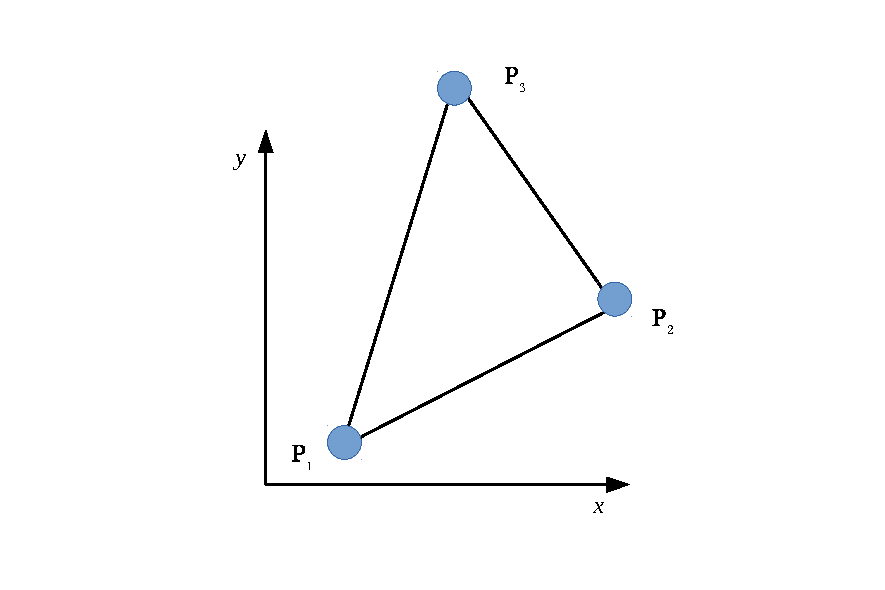
\includegraphics[scale=.8]{triangulo_simple}
\caption{\label{fig:tri_simple} Triángulo formado por tres puntos $ \lbrace \vec{P}_{1}, \vec{P}_{2}, \vec{P}_{3}  \rbrace $}
\end{figure}

Además, cada uno de ellos puede contener información relativa a cualquier cantidad fisica de interés, es decir, sobre $ \vec{P}_{1} $ por ejemplo, podría encontrarse definida una cantidad vectorial cualquiera $ \vec{v}_{1}$, y para el resto de los puntos cualquier otra cantidad $ \vec{v}_{i=2,3} $. Por lo tanto, si sólo se conocen las magnitudes físicas sobre tales posiciones espaciales, ¿cómo podremos hallar la cantidad $ \vec{v}_{p} $ correspondiente a un punto $\vec{p}$ que se encuentre dentro del triángulo definido por $ \lbrace \vec{P}_{1}, \vec{P}_{2}, \vec{P}_{3}  \rbrace $? Para responder a ésto, utilizamos un método de interpolación que consiste en la utilización de coordenadas de áreas, también denominadas coordenadas baricentricas, para luego obtener $ \vec{v}_{p} $ simplemente ponderando cada $ \vec{v}_{i=1,2,3} $ de acuerdo a su posición relativa a $ \vec{p} = \lbrace x,y \rbrace $, como se muestra en la ecuación (\ref{eq:combinacionlinealtrixy}).
%%%%%%%%%%%%%%%%%%%%%%%%%%%%%%%%%%
\begin{equation}
\label{eq:combinacionlinealtrixy}  
  \vec{v}_{p} = 
  N_{1}(\vec{p}) \cdot \vec{v_1} + 
  N_{2}(\vec{p}) \cdot \vec{v_2} + 
  N_{3}(\vec{p}) \cdot \vec{v_3} 
\end{equation}
%%%%%%%%%%%%%%%%%%%%%%%%%%%%%%%%%%
Las funciones de (\ref{eq:combinacionlinealtrixy}), $ N_{i} ( \vec{p} )$, se denominan funciones de forma y deben hallarse de tal manera que, cuando $ \vec{p} = \vec{P}_{i} $, la salida de (\ref{eq:combinacionlinealtrixy}) sea exactamente $\vec{v}_{i}$.\\
Si bien es correcto trabajar con las funciones $ N_{i} ( \vec{p} )$ basadas en las coordenadas $(x,y)$, nosotros hemos decidido realizar un cambio de variables, ya que realizamos un mapeo de las coordenadas definidas en el plano $(x,y)$, hacia coordenadas $ (\xi, \eta) \in [0, 1] $ (ver figura \ref{fig:tri}).

\begin{figure}
\centering
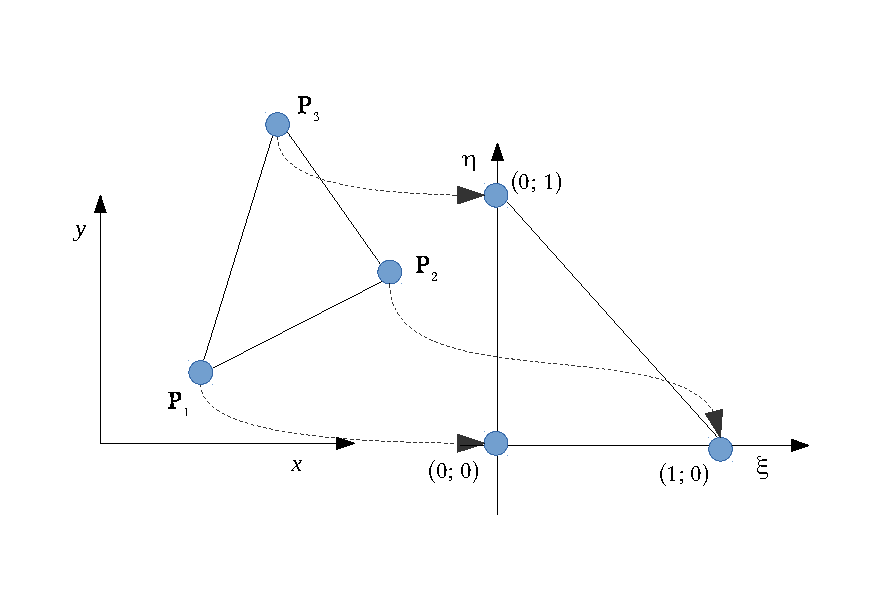
\includegraphics[scale=.8]{Triangulo}
\caption{\label{fig:tri} } Mapeo de un triángulo definido en $(x,y)$ a $(\xi, \eta) \in [0; 1]$.
\end{figure}

 Entonces, para cualesquiera 3 puntos $ \lbrace \vec{P}_{1}, \vec{P}_{2}, \vec{P}_{3}  \rbrace $, tendremos que el mapeo nos producirá las relaciones definidas en (\ref{eq:verticesmastertri}).

%%%%%%%%%%%%%%%%%%%%%%%%%%%%%%%%%%
\begin{equation}
  \label{eq:verticesmastertri}
  \vec{P_1} \rightarrow 
  \begin{bmatrix}
    0\\ 
    0
  \end{bmatrix}\quad \vec{P_2} \rightarrow
  \begin{bmatrix}
    1\\
    0
  \end{bmatrix}\quad \vec{P_3} \rightarrow
  \begin{bmatrix}
    0\\
    1
  \end{bmatrix}
\end{equation}
%%%%%%%%%%%%%%%%%%%%%%%%%%%%%%%%%%

La ventaja de llevar a cabo el cambio de variables, radica en que podremos tratar a todo triángulo definido por tres puntos cualquiera, como un único triángulo estandar (denominado elemento máster), que se encuentra acotado al intervalo $ [0; 1] $. En futuras aplicaciones de ésta técnica, se hará visible con mayor facilidad la ventaja, ya que a la hora de llevar a cabo integraciones numéricas, éstas operaciones no dependerán de la forma del triángulo, sino que harán uso del elemento máster. 
\\
Ahora, teniendo en cuenta (\ref{eq:verticesmastertri}), vemos que las coordenadas $x$ e $y$, necesitan relacionarse funcionalmente con  $\xi$ y $\eta$, y lo inverso también es cierto, es decir: $x=x( \xi, \eta)$; $y=y( \xi, \eta)$; $\xi= \xi(x,y)$ y $\eta= \eta(x,y)$. Éstas relaciones son importantes, ya que nos permiten trasladarnos de un espacio a otro, pero por el momento estamos interesados en determinar $\xi= \xi(x,y)$ y $\eta= \eta(x,y)$, para luego evaluar las funciones de forma sobre los parámetros $(\xi, \eta)$. Sin profundizar en su obtención, llegamos a
 
%%%%%%%%%%%%%%%%%%%%%%%%%%%%%%%%%%
\begin{equation}
  \label{eq:chietadexy}
  \begin{split}
    \xi(x,y) & =
    \frac{x(y_3-y_1)+y(x_1-x_3)+y_1x_3-y_3x_1}{(x_2-x_1)(y_3-y_1)+(y_1-y_2)(x_3-x_1)} \\
    \eta(x,y) & =
    \frac{x(y_1-y_2)+y(x_2-x_1)+y_2x_1-y_1x_2}{(x_2-x_1)(y_3-y_1)+(y_1-y_2)(x_3-x_1)}
  \end{split}
\end{equation}
%%%%%%%%%%%%%%%%%%%%%%%%%%%%%%%%%%

Por otra parte, con las consideraciones mencionadas anteriormente y sin ahondar en los pasos algebraicos necesarios, llegamos a obtener las siguientes igualdades para las funciones de forma.

%%%%%%%%%%%%%%%%%%%%%%%%%%%%%%%%%%
\begin{equation}
  \label{eq:fftridechieta}
  \begin{split}
    N_1(\xi,\eta) & = 1 - \xi - \eta \\
    N_2(\xi,\eta) & = \xi            \\
    N_3(\xi,\eta) & = \eta           
  \end{split}
\end{equation}
%%%%%%%%%%%%%%%%%%%%%%%%%%%%%%%%%%
Así, (\ref{eq:combinacionlinealtrixy}) se puede reescribir como sigue.
%%%%%%%%%%%%%%%%%%%%%%%%%%%%%%%%%%
\begin{equation}
  \label{eq:combinacionlinealtrichieta}  
  \begin{split}
    \vec{v} & = 
    N_{1}(\xi,\eta) \cdot \vec{v_1} + N_{2}(\xi,\eta) \cdot \vec{v_2}
    + N_{3}(\xi,\eta) \cdot \vec{v_3} \\
    & = (1-\xi-\eta) \cdot \vec{v_1} + \xi\vec{v_2} + \eta\vec{v_3}
    \end{split}
\end{equation}
%%%%%%%%%%%%%%%%%%%%%%%%%%%%%%%%%%
Con éstas simples ecuaciones, ahora es posible determinar, cuál es el valor de la magnitud física que se desea medir sobre el punto $\vec{p}$ perteneciente al triángulo en cuestión.
\\
Una situación que debemos tener en cuenta es cuando el punto $\vec{p}$ no se encuentra dentro del triángulo mencionado. En primer lugar, para determinar si el punto pertenece o no a dicha figura geométrica, debemos analizar las coordenadas $\xi= \xi(x,y)$ y $\eta= \eta(x,y)$. El procedimiento de verificación, básicamente, es el siguiente: cuando $\xi$ o $\eta$ son menores que cero ya podemos descartar el hecho de que $\vec{p}$ se encuentre en el interior de triangulo; si se encuentran por encima de la recta definida por $1-\xi-\eta$ entonces tampoco pertenece al triangulo; así, en cualquier otro caso, el punto está en el interior de la figura. 

\subsection{El caso del cuadrilátero}
\label{sec:cuadrilatero}
Como en el caso del triángulo, cuando es conocida una magnitud física sobre los vertices de un cuadrlátero definido por los puntos $ \lbrace \vec{P}_{1}, \vec{P}_{2}, \vec{P}_{3}, \vec{P}_{3}  \rbrace $, puede hallarse el valor numérico en cualquier punto del interior de la figura haciendo
%%%%%%%%%%%%%%%%%%%%%%%%%%%%%%%%%%
\begin{equation}
\label{eq:combinacionlinealcuaxy}  
  \vec{v} = 
  N_{1}(\vec{p}) \cdot \vec{v_1} + 
  N_{2}(\vec{p}) \cdot \vec{v_2} + 
  N_{3}(\vec{p}) \cdot \vec{v_3} +  
  N_{4}(\vec{p}) \cdot \vec{v_4} 
\end{equation} 
%%%%%%%%%%%%%%%%%%%%%%%%%%%%%%%%%%
Como puede observarse, ésta forma de calcular $ \vec{v}_{p} $ es similar a la utilizada para el triángulo, sólo que debe añadirse un término más para contemplar la presencia de un vértice adicional.
\\
También, llevamos a cabo un cambio de variables, pero aquí las nuevas variables $(\xi, \eta)$ van a estar contenidas en la región cuadrada $[-1;1]$. Así, estamos mapeando un cuadrilatero de forma irregular a un cuadrado estandar de magnitud 2 en sus lados y centrado en el origen (características deseables para llevar a cabo integracion numérica mediante cuadratura Gaussiana sobre una tal región)  (ver figura \ref{fig:cuad}). 

\begin{figure}
\centering
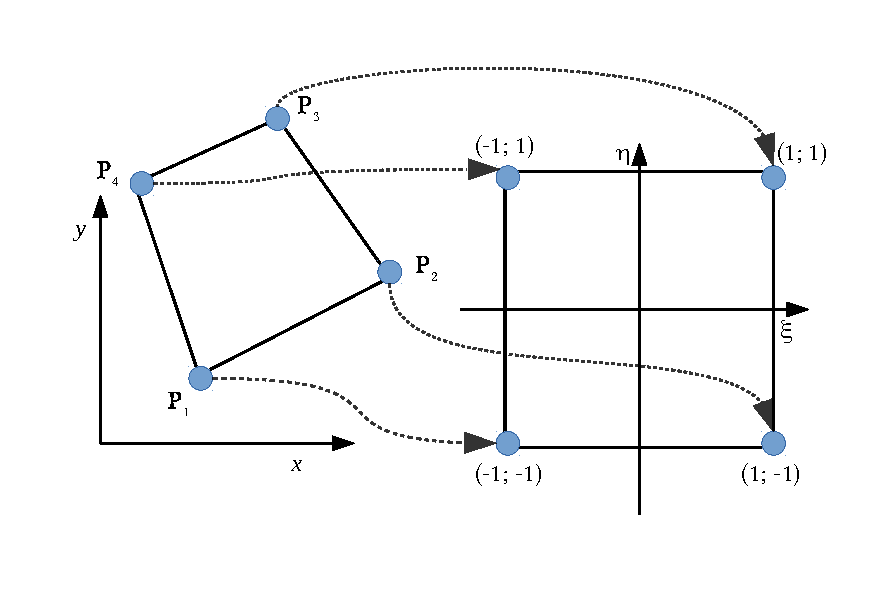
\includegraphics[scale=.8]{Cuadrilatero}
\caption{\label{fig:cuad} } Mapeo de un cuadrilátero definido en $(x,y)$ a $(\xi, \eta) \in [-1; 1]$.
\end{figure}

Para poder mapear puntos definidos sobre el plano $(x,y)$ al plano $(\xi, \eta)$, es necesario resolver el sistema dado por 

%%%%%%%%%%%%%%%%%%%%%%%%%%%%%%%%%%
\begin{equation}
  \label{eq:mapeoinversocuadrado}
  \begin{split}
    x & = a_1 + a_2\xi + a_3\eta + a_4\xi\eta \\
    y & = b_1 + b_2\xi + b_3\eta + b_4\xi\eta
  \end{split}
\end{equation}
%%%%%%%%%%%%%%%%%%%%%%%%%%%%%%%%%%
Donde $(a_1, b_1)= \frac{(\vec{P_1} + \vec{P_2} + \vec{P_3} +
  \vec{P_4})}{4}$; $(a_2, b_2)=  \frac{(\vec{P_2} - \vec{P_1} + \vec{P_3} -
  \vec{P_4})}{4}$; $(a_3, b_3)= \frac{(\vec{P_3} - \vec{P_2} + \vec{P_4} -
  \vec{P_1})}{4} $; $(a_4, b_4)= \frac{(\vec{P_1} - \vec{P_2} + \vec{P_3} - \vec{P_4})}{4}$. \\ \\
Como la forma cerrada de $\xi= \xi(x,y)$ y $\eta= \eta(x,y)$ que se obtiene al resolver (\ref{eq:mapeoinversocuadrado}) es algo extensa, preferimos no incluirlas para mantener la legibilidad del documento. \\
Nuevamente, para determinar si un punto dado definido en el plano $(x,y)$ se encuentra dentro del cuadrado $[-1; 1]$, es necesario aplicar un método de verificación sencillo: básicamente, si [$(\xi$, $\eta) <  -1$] ó [$(\xi$, $\eta) >  1  $], el punto no se encuentra dentro del cuadrilátero y no deberá calcularse ninguna magnitud sobre él. En cuanto a las funciones de forma, las cuales se modifican para calcularse sobre las nuevas variables $(\xi, \eta)$, poseen las siguientes expresiones.

%%%%%%%%%%%%%%%%%%%%%%%%%%%%%%%%%%
\begin{equation}
  \label{eq:ffcuadechieta}
  \begin{split}
    N_1 & = \frac{ (1-\eta)(1-\xi) }{4} \\
    N_2 & = \frac{ (1+\eta)(1-\xi) }{4} \\
    N_3 & = \frac{ (1+\eta)(1+\xi) }{4} \\
    N_4 & = \frac{ (1-\eta)(1+\xi) }{4} 
  \end{split}
\end{equation}
%%%%%%%%%%%%%%%%%%%%%%%%%%%%%%%%%%

Las funciones de forma en (\ref{eq:ffcuadechieta}) permiten modificar a la ecuación (\ref{eq:combinacionlinealcuaxy}), para reescribbirla de la siguiente manera:

\begin{equation}
\label{eq:vdechieta}  
  \vec{v} = 
  \frac{ (1-\eta)(1-\xi) }{4} \cdot \vec{v_1} + 
  \frac{ (1+\eta)(1-\xi) }{4} \cdot \vec{v_2} + 
  \frac{ (1+\eta)(1+\xi) }{4} \cdot \vec{v_3} +  
  \frac{ (1-\eta)(1+\xi) }{4} \cdot \vec{v_4} 
\end{equation} 

\section{Aplicación de desenrollado de ciclos}
\label{sec:desenrollado}

En esta sección se pondrá en manifiesto como aplicar la técnica de
desenrollado de ciclos en un algoritmo. La misma consiste en, dado un
ciclo iterativo común y corriente, disminuir la cantidad de
repeticiones mediante la codificación explícita de algunas o todas las
iteraciones. Esta técnica produce una mejora significativa en el
tiempo de ejecución del algoritmo, como lo veremos en el siguiente
ejemplo.

Supongamos que tenemos una matriz de Nx3, donde cada fila contiene un
vector en el espacio tridimensional. Ahora supongamos que necesitamos
un algoritmo que calcule el módulo de cada vector que está almacenado
en esta matriz, y que el resultado se almacene en un vector de
Nx1. Este algoritmo podría implementarse en C++ de la siguiente
manera:

 
Para aplicar el método de desenrollado de ciclos, podríamos
deshacernos del ciclo interno simplemente escribiendolo de manera
explícita como se hizo en la función
\emph{modulos\_vectores\_desenrollado}:


A continuación se hará una prueba comparativa de estos dos algoritmos,
con matrices de tamaño 10, 100, y 1000. Los resultados de los tiempos
de ejecución pueden verse en la tabla \ref{tab:resultados}, donde
podemos observar que el desenrollado tiene un desempeño
notablemente mejor considerando el tiempo de ejecución.

\begin{table}[H]
  \centering
  \begin{tabular}{l|r}
    Sin desenrollado & Con desenrollado \\\hline
    1.9E-05 & 1E-05 \\
    1.13E-04 & 8.1E-05 \\
    8.71E-04 & 6.57E-04
  \end{tabular}
  \caption{\label{tab:resultados}Tabla comparativa de tiempos de
    ejecución en segundos.}
\end{table}

\section{Conclusiones}

Haciendo un análisis de los resultados obtenidos en las secciones
\ref{sec:matrices} y \ref{sec:desenrollado} podemos concluir que las
técnicas de reordenamiento y desenrollado de ciclos son muy útiles a
la hora de programar, ya que en este informe se ha puesto en evidencia
mediante sencillos ejemplos que los tiempos de ejecución mejoran
notablemente cuando se utilizan las mismas. Además, estos tiempos de
ejecución podrían mejorarse aun mas si se aplicaran ambas técnicas de
manera simultánea o si se complementaran con otras técnicas que se han
visto a lo largo de esta unidad temática.

 \end{document}


% \begin{figure}
 %   \centering
%   \includegraphics[width=1.0\textwidth]{resultados.eps}
%   \caption{\label{fig:reporte-ORNL}Reporte a enviar a la ORNL: ejemplo
%   1000d}
% \end{figure}

% \subsection{Tables and Figures}

% Use the table and tabular commands for basic tables --- see
% Table~\ref{tab:widgets}, for example. You can upload a figure (JPEG,
% PNG or PDF) using the files menu. To include it in your document,
% use the includegraphics command as in the code for
% Figure~\ref{fig:frog} below.

% % % Commands to include a figure:
% % \begin{figure}
% % \centering
% % \includegraphics[width=0.5\textwidth,natwidth=399,natheight=356]{curva.jpg}
% % \caption{\label{fig:frog}This is a figure caption.}
% % \end{figure}

% % \begin{table}
% % \centering
% % \begin{tabular}{l|r}
% % Item & Quantity \\\hline
% % Widgets & 42 \\
% % Gadgets & 13
% % \end{tabular}
% % \caption{\label{tab:widgets}An example table.}
% % \end{table}

% \subsection{Matematicas}

% \LaTeX{} is great at typesetting mathematics. Let $X_1, X_2, \ldots,
% X_n$ be a sequence of independent and identically distributed random
% variables with $\text{E}[X_i] = \mu$ and $\text{Var}[X_i] = \sigma^2
% < \infty$, and let
% $$S_n = \frac{X_1 + X_2 + \cdots + X_n}{n}
% = \frac{1}{n}\sum_{i}^{n} X_i$$ denote their mean. Then as $n$
% approaches infinity, the random variables $\sqrt{n}(S_n - \mu)$
% converge in distribution to a normal $\mathcal{N}(0, \sigma^2)$.

% \subsection{Lists}

% You can make lists with automatic numbering \dots

% \begin{enumerate}
% \item Like this,
% \item and like this.
% \end{enumerate}
% \dots or bullet points \dots
% \begin{itemize}
% \item Like this,
% \item and like this.
% \end{itemize}

% We hope you find write\LaTeX\ useful, and please let us know if you
% have any feedback using the help menu above.


%%% Local Variables: 
%%% mode: latex
%%% TeX-master: t
%%% End: 
